\chapter{Historia}
\section{Scauting}
\begin{floatingfigure}[r]{3cm}
\centering
  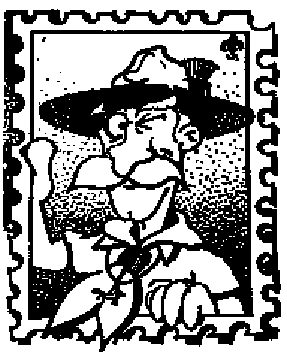
\includegraphics[width=3cm]{grafiki/bp.png}
\end{floatingfigure}
Twórcą skautingu jest gen. Robert Stephenson Smyth Baden - Powell. 
B-P urodził się w Londynie jako syn profesora na Uniwersytecie Oksfordzkim. 
To ten pogodny mężczyzna po lewej stronie. 
W dzieciństwie wiele czasu spędzał w gąszczu londyńskiego Hyde Parku, gdzie z pasją oddawał się podchodom. 
Wybierał się też często do dzielnic nędzy, rozmyślając o losie żyjących tam ludzi. 
Doszedł do wniosku, że tym, co najbardziej dzieli biednych od bogatych jest ich lichy strój, który pozwala na pierwszy rzut oka rozpoznać pochodzenie człowieka.

Jako młodzieniec skończył szkołą oficerską i rozpoczął służbę w Indiach. Będąc porucznikiem musiał szkolić rekrutów. 
Wkrótce zauważył, że kompania żołnierzy reaguje jak maszyna - obojętnie i bezmyślnie - i nie ma tu mowy o inicjatywie indywidualnej. 
Podzielił ją więc na patrole, a na dowódców wyznaczył najzdolniejszych żołnierzy. 
Pozwolił im popełniać błędy, by zachęcić ich do działania, lecz przestrzegał ich przed popełnieniem tego samego błędu dwa razy. Sam szkolił dowódców patroli, oni zaś - swoich żołnierzy. 
Później system ten zyskał uznanie i został wprowadzony w całym wojsku brytyjskim! 
Przebywając w Indiach wciąż jako porucznik doprowadził do wprowadzenia do armii nowego typu wywiadu, który został nazwany scoutingiem.

Zwiadowcy Baden-Powella początkowo byli namawiani do niepalenia, później niepalenie stało się warunkiem zostania zwiadowcą (zwiadowca musiał mieć sprawny \\ węch). 
Skuteczność scoutingu udowodnił, kiedy jego garnizon wygrał manewry z wojskami pułkownika Temple - właśnie dzięki nowym metodom wywiadowczym. 
Swoje metody oparł na obserwacjach hinduskich tropicieli i myśliwych oraz na własnych doświadczeniach z dziecięcych i młodzieńczych zabaw z braćmi. Wojsko poleciło mu napisać podręcznik, który nazwał Służba rozpoznania i łączności. 
Od tego czasu zajmował się szkoleniem zwiadowców. 
Niedługo potem w Afryce, już jako kapitan, B-P był świadkiem śmierci małej Zuluski, postrzelonej nieumyślnie przez wojsko. 
Później domagał się wprowadzenia do wojska szkolenia z zakresu pierwszej pomocy. 
Kierując budową drogi i mostów prowadzących przez dżunglę do pewnej twierdzy, zauważył, że wśród pracujących dla niego tubylców pewna część wyróżniała się. 
Ci ludzie witali się przez podawanie sobie lewej ręki. 
Okazało się, że stanowią oni pewien rodzaj elity wśród swojego plemienia. Ich powitanie stało się później powitaniem wszystkich skautów. 
Udoskonalał wciąż metody zwiadowcze, opierając się na obserwacji afrykańskich wojowników. Wydał nowy podręcznik wojskowy Poradnik scoutingu.

Bardzo ważnym wydarzeniem była obrona Mafekingu przed wojskami burskimi. Baden - Powell jako pułkownik dowodził dziesięciokrotnie mniejszym oddziałem od wojsk oblężniczych. 
\begin{wrapfigure}{r}{3cm}
  \begin{center}
    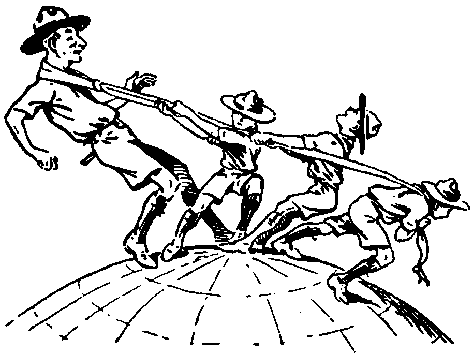
\includegraphics[width=2.9cm]{grafiki/bardzo.png}
  \end{center}
\end{wrapfigure}
Musiał więc do służby zaangażować także młodych chłopców. Zadziwiło go, że sprawowali się oni w sposób nadspodziewanie odpowiedzialny. Doszedł do wniosku, że chłopiec, który dostanie odpowiedzialne zadanie, spełni je niejednokrotnie lepiej od regularnego żołnierza. Obrona Mafekingu dzięki nieziemskiemu sprytowi Baden-Powella zakończyła się sukcesem Brytyjczyków. B-P jeszcze przed powrotem do Anglii usłyszał od brata, który przybył do Mafekingu jako major, interesującą wiadomość. Mianowicie, jego drugi podręcznik Poradnik skautingu, który był obowiązkową lekturą każdego żołnierza, zyskał niesamowitą popularność wśród młodzieży. Według relacji brata młodzi chłopcy masowo wyjeżdżali za miasto i tam odbywali wędrówki wykorzystując całą wiedzę zawartą w podręczniku B-P. On sam zawsze zadawał sobie pytanie jak uniknąć wojen. I wydało mu się, że teraz znalazł klucz, że wzrastający w obcowaniu z przyrodą młodzi chłopcy wyrastają na innych ludzi niż ci tkwiący w wielkim mieście, że gry na orientację wyrabiają postawę dążenia do celu, co odbije się postawą konsekwencji w dorosłym życiu.

B-P wrócił do Londynu jako bohater i wyzyskując sprzyjającą sytuację zajął się organizacją ruchu młodzieżowego, który nazwał skautingiem. Na jego kształt wpłynęły opisane fakty z jego życia: opierał się na systemie małych grup (zastępy), kontakcie z przyrodą, powierzaniu odpowiedzialności młodym ludziom. Wprowadził do niego szkolenie pierwszej pomocy i mundur, który zacierał różnice między biednymi i bogatymi. Przeredagował też swój wojskowy podręcznik tak, by mógł służyć młodzieży i wydał go pod nazwą Skauting dla chłopców. Organizacją ruchu skautowego zrealizował także swoje dawne marzenie zmiany surowego wiktoriańskiego modelu wychowania. Pierwszy obóz skautowy odbył się w 1907 roku na wyspie Brownsea u wybrzeża Wielkiej Brytanii w okolicy portu Poole. W 1909 roku w Anglii odbył się pierwszy zlot skautowy z udziałem 11.000 uczestników. W 1912 ukazał się pierwszy żeński podręcznik skautowy. W 1920 w Londynie odbył się I Zlot Międzynarodowy Jamboree . B-P został na nim uznany przez wszystkie światowe organizacje skautowe Skautem Naczelnym Świata. Przez ojczyznę został obdarzony tytułem lorda. B-P zmarł w 1941 roku w Kenii. 

\section{Powstanie harcerstwa w Polsce. harcerstwo w II Rzeczypospolitej}

Jesienią 1909 roku niemal jednocześnie w dwóch czasopismach (warszawskim i lwowskim) ukazały się artykuły informacyjne o nowym ruchu wychowawczym, który zdobył sobie niezwykłą popularność wśród młodzieży angielskiej (mowa o skautingu). Metody skautowe zwróciły uwagę działaczy Zarzewia (Henryk Bagiński, Andrzej Małkowski – to ten po lewej, Neugebauer) - tajnej młodzieżowej organizacji paramilitarnej przygotowującej swych członków do walki o niepodległość Polski.\begin{wrapfigure}{l}{3cm}
  \begin{center}
    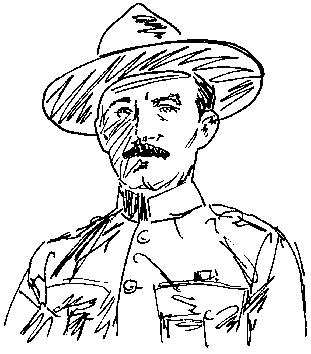
\includegraphics[width=2.9cm]{grafiki/malkowski.png}
  \end{center}
\end{wrapfigure} Władze Zarzewia zleciły Andrzejowi Małkowskiemu przetłumaczenie angielskiego podręcznika Scouting for boys. Szybko stał się on entuzjastą skautingu, uważając go za nowy styl życia.
Małkowski był także członkiem towarzystwa gimnastycznego Sokół we Lwowie - potężnej wówczas organizacji, jawnej, działającej w trzech zaborach (w rosyjskim tajnej), mającej własną sieć sal gimnastycznych. Był również członkiem Stowarzyszenia Eleusis propagującego poczwórną wstrzemięźliwość - od alkoholu  i tytoniu. To właśnie tej organizacji zawdzięczamy 10. punkt Prawa Harcerskiego, ewenement na skalę światową oraz patriotyczno-narodowy charakter harcerstwa. Małkowski wciągnął do współpracy innych członków tego stowarzyszenia - Wincentego Lutosławskiego, Tadeusza Strumiłłę, Jerzego Grodyńskiego, Jadwigę Falkowską, Olgę Drahonowską (swoją przyszłą żonę) i wielu innych. Zarzewiacy, elsowie, wszyscy uczestnicy kursu chłonęli informacje o skautingu. 21. maja 1911 r. powstała Komenda Skautowa we Lwowie. W dzień później A. Małkowski wydał rozkaz o powołaniu pierwszych drużyn: trzech męskich i jednej żeńskiej. W lipcu 1911 r. ukazała się pierwsza polska książka skautowa: Skauting jako system wychowania młodzieży na podstawie gen. Roberta Baden-Powella <<Scouting for boys>> przedstawił Andrzej Małkowski. 15. października wyszedł we Lwowie pierwszy numer dwutygodnika Skaut z wierszem Wszystko co nasze... na stronie tytułowej, redagowany przez Małkowskiego. Na bibułach (powszechnie stosowaną konspiracyjną metodą), podobnie jak książka Małkowskiego, Skaut docierał do wszystkich zaborów. Skauting ze Lwowa promieniował na cały, choć podzielony, kraj. W grudniu utworzono w Warszawie Naczelną Komendę Skautową na Królestwo Polskie (część zaboru rosyjskiego).

W lutym 1912 roku na łamach Skauta rozstrzygnięty został konkurs na polską odznakę skautową, ogłoszony w jego pierwszym numerze. Żadna z prac nie wydała się na tyle interesująca, by od razu wprowadzić ją do użytku, toteż w końcu roku NKS wyznaczyła do dalszych prac nad projektem ks. Kazimierza Lutosławskiego z zespołem, którego praca zdobyła w konkursie III nagrodę. Jego projekt wzorowany był na orderze Virtuti Militari. Po wprowadzeniu w nim szeregu zmian, Krzyż Harcerski zaprojektowany przez ks. Lutosławskiego wszedł do użytku w 1913 roku. To właśnie na nim po raz pierwszy w Polsce znalazła się lilijka harcerska, wzorowana na lilijce skautowej. 24 - 25 marca 1912 roku odbył się pierwszy zjazd drużyn i plutonów harcerskich. Przybyło na niego 100 uczestników. W czerwcu 1912 ukazała się znana polska książka Eugeniusza Piaseckiego i Mieczysława Schreibera Harce młodzieży polskiej, w której po raz pierwszy użyto staropolskiej terminologii rycerskiej, czyli wyrazów takich, jak: harcerz (zastąpił określenie skaut polski), zastęp (zastąpił określenie pluton), drużyna, hufiec, harce (oznaczające kiedyś ćwiczenia rycerstwa przed bitwą). Zaproponowano w niej także używane do dziś nazwy stopni i funkcji (wyraz chorągiew również należy do dawnej terminologii rycerskiej).

2. lipca 1913 roku 43 skautów z trzech zaborów wyjechało na III Wszechbrytyjski Zlot Skautów w Birmingham. Mieli tam obóz pod polską flagą! Tuż przed wybuchem I wojny światowej polski skauting liczył ponad 15.000 członków. Już wtedy tworzono polskie harcerstwo poza (wtedy jeszcze historycznymi) granicami kraju. Podczas całej wojny skauci brali udział w bardzo wielu akcjach pomocniczych i zbrojnych. Konflikty polityczne spowodowane wybuchem wojny podzieliły skautów na kilka organizacji. Jednak w Królestwie Polskim wobec utrudniania działalności harcerstwa przez władze, organizacje harcerskie postanowiły się zjednoczyć. 1 i 2 listopada 1916 roku w Warszawie w efekcie zjednoczenia wszystkich organizacji harcerskich zaboru rosyjskiego powstaje Związek Harcerstwa Polskiego. Do zjednoczenia harcerstwa wszystkich zaborów doszło na zjeździe w Lublinie 1 i 2 listopada 1918 roku, gdy na ulicach miast rozpoczęło się już rozbrajanie wrogich wojsk. Oficjalnie przyjęto na nim nazewnictwo zaproponowane przez Piaseckiego i Schreibera. Harcerstwo liczyło wtedy już ok. 30~000 członków. W nocy z 15 na 16 stycznia 1919 roku w katastrofie morskiej w Cieśninie Messyńskiej zginął Andrzej Małkowski. Od 31. grudnia 1920 do 2. stycznia 1921 roku obradował w Warszawie I Walny Zjazd ZHP, na którym przyjęto statut ZHP. 
\begin{wrapfigure}{l}{3cm}
  \begin{center}
    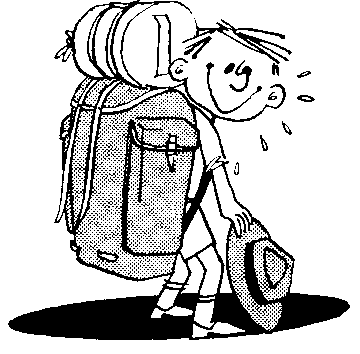
\includegraphics[width=2.9cm]{grafiki/lipca.png}
  \end{center}
\end{wrapfigure}
4 - 9 lipca 1924 odbyły się pierwsze narodowe zloty: harcerzy na Siekierkach i harcerek w Świdrze. Po odzyskaniu niepodległości zwrócono uwagę na dominujący, nadmiernie rozbudowany w harcerstwie militaryzm, który wówczas nie był już potrzebny. Szukano sposobu wyjścia z kryzysu. Stworzono więc programy specjalnościowe, które okazały się świetnym na niego lekarstwem. Rozwijało się harcerskie szybownictwo, żeglarstwo, kajakarstwo, turystyka kwalifikowana, krótkofalarstwo, strzelectwo, spadochroniarstwo, rozmaite kluby sportowe. Harcerstwo kwitło dzięki dużemu wsparciu finansowemu państwa. Punktem kulminacyjnym jego rozwoju okazał się słynny zlot w Spale 11 - 27 lipca 1935 roku. Wzięło w nim udział 25~000 uczestników. Wcześniej, poczynając od 1933 roku, Aleksander Kamiński rozpoczął rozwój zuchostwa. Choć pierwszą drużynę zorganizowała w 1914 roku w Zakopanem Olga Małkowska, wzorując się na brytyjskich Wilczętach, dopiero Kamiński znalazł odpowiednie rozwiązania metodyczne i uczynił z ruchu zuchowego poważną gałąź działalności harcerstwa. W końcu 1938 roku dwie części składowe ZHP - Organizacja Harcerzy i Organizacja Harcerek liczyły odpowiednio 130~500 i 71~600 członków. We wrześniu 1938 roku w związku z akcją zajęcia przez wojsko polskie Zaolzia utworzono Pogotowie Harcerek z odrębną siecią podległości pod komendanturą hm. Józefiny Łapińskiej. Po zakończeniu operacji nie zostało ono zlikwidowane. Trwały szkolenia sanitarne, łącznościowe, przeciwlotnicze i przeciwgazowe.

\section{Harcerstwo podczas II wojny światowej}

Wiele było przykładów udziału harcerzy w działaniach wojennych Kampanii Wrześniowej. U jej kresu, 27 września 1939 roku w Warszawie (w dniu jej kapitulacji), na naradzie obecnych w Warszawie członków Naczelnej Rady Harcerskiej i innych wybitnych instruktorów zapadła decyzja o kontynuowaniu działalności harcerstwa w konspiracji. Naczelnikiem harcerstwa męskiego wybrano hm. Floriana Marciniaka (ps. Nowak), który miał je zorganizować i stworzyć jego program, przyjmując dla niego kryptonim Szarych Szeregów. Kryptonimy jednostek organizacyjnych były następujące: Kwatera Główna - Pasieka, chorągwie - Ule, hufce - Roje, drużyny - Rodziny, zastępy - Pszczoły. Harcerki miały działać w zorganizowanym już Pogotowiu Harcerek, które występowało pod kryptonimem Związek Koniczyn, Szare Szeregi żeńskie, a później Bądź gotów. Część dziewcząt działało w organizacji męskiej w rozmaitych służbach pomocniczych oddziałów, a zwłaszcza w służbach sanitarnej i łączności. W wyżej wymienionych oraz w różnych służbach cywilnych (opieka nad dziećmi, pomoc więźniom, jeńcom i ich rodzinom, pomoc ludziom starym i chorym, Żydom, tajne nauczanie) działało Pogotowie Harcerek, a później Związek Koniczyn. Pełniły one te funkcje zarówno we wrześniu 1939 r., w czasie okupacji, jak i podczas Powstania Warszawskiego. Gdy w lutym 1942 roku powstał Referat Wojskowej Służby Kobiet AK (a była ona organizowana już od października 1939), harcerki powyżej 16 lat były przekazywane do jego dyspozycji. Zastępczyniami komendantki WSK były instruktorki harcerskie - Jadwiga Falkowska i Ewa Grodecka. Pierwszym zadaniem dowództwa Szarych Szeregów była konsolidacja oraz integracja organizacji, istniało bowiem wiele realizujących własny program drużyn, wiele związało się z mnożącymi się wówczas tajnymi organizacjami (między innymi słynna później szaroszeregowa 23. WDH Pomarańczarnia Zośki). Aby wyeliminować problem masowego odchodzenia starszych harcerzy do oddziałów wojskowych, organizowano im uczestnictwo w szkoleniach i służbach Związku Walki Zbrojnej (późniejszej Armii Krajowej) nie zmieniając ich przynależności organizacyjnej. Kłopotem był brak szkolnictwa ponadpodstawowego, przez co młodzież organizowała się w kręgi samokształceniowe stanowiące konkurencję dla harcerstwa.

W grudniu 1940 roku Aleksander Kamiński sformułował program akcji Wawer, który znalazł szeroki odzew wśród całej, nie tylko harcerskiej, młodzieży (poza organizacją nawet wśród dzieci). 
Nazwa pochodziła od nazwy podwarszawskiej wówczas miejscowości, gdzie w grudniu 1939 roku okupant dokonał pierwszej masowej zbrodni w rejonie Warszawy mordując ponad 100 ludzi wywleczonych z domów w odwecie za śmierć niemieckiego żołnierza zamordowanego przez kryminalistów. 
\begin{wrapfigure}{l}{3cm}
  \begin{center}
    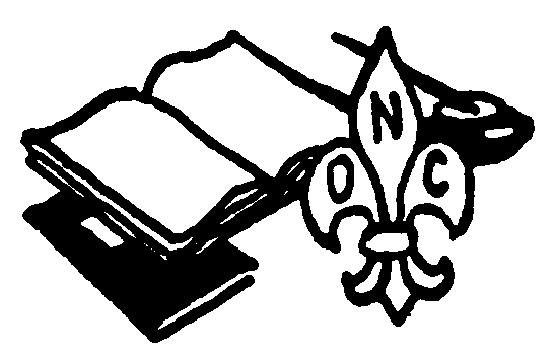
\includegraphics[width=2.9cm]{grafiki/onc.png}
  \end{center}
\end{wrapfigure}Dla warszawiaków nazwa ta wyrażała nienawiść do najeźdźcy. Początkowo Wawer polegał na płataniu figli, częstokroć bardzo dokuczliwych, Niemcom i polskim zdrajcom (szykany, napisy na murach, ulotki, wybijanie szyb). Później mały sabotaż podejmował także trudniejsze zadania - gazowanie kin, wywieszanie polskich flag, nadawanie polskich audycji przez niemiecką sieć radiową, kolportaż polskich dodatków do wydawanej przez Niemców prasy, rozmaite akcje propagandowe. Akcja Wawer w ciągu całego roku 1941 znacząco przyczyniła się do pokonania problemów Szarych Szeregów, z czasem przestała jednak wystarczać starszej młodzieży. Jej wejściu do struktur wojskowych sprzyjało przekształcenie ZWZ w AK, gdzie zaszły istotne zmiany w formach i kierunkach działania wojska. Po uregulowaniu stosunku Sz. Sz. i AK (rozkaz Komendanta Głównego AK z marca 1942 r.) starsza młodzież miała współistnieć jednocześnie w obu organizacjach, młodsza miała brać udział jedynie w szkoleniach i służyć w służbach pomocniczych. W połowie 1942 roku wprowadzono ostatecznie program Sz. Sz. Dziś – Jutro - Pojutrze. Dziś oznaczoło walkę konspiracyjną, Jutro - powstanie, Pojutrze - wolną Polskę. Każda z wyodrębnionych wkrótce grup wiekowych w inny sposób realizowała walkę Dziś oraz przygotowywała się do walki Jutro i pracy w wolnej Polsce Pojutrze. Pojutrze miało zapobiegać całkowitej militaryzacji młodzieży, sprawić, aby była ona gotowa do życia w kraju po wojnie, aby wojna nie zrobiła z niej wraków niezdolnych do życia w normalnych warunkach. Zawiszacy realizowali lżejsze formy akcji Wawer, rozprowadzali prasę, zajmowali się łatwiejszymi formami łączności i wywiadu (na Dziś), byli szkoleni do służby pomocniczej (na Jutro) oraz uczyli się w szkole, oprócz niemieckiej podstawówki na tajnych kompletach uczyli się nieobecnych w niej przedmiotów: języka polskiego, geografii, historii; starsze roczniki uczyły się w szkołach zawodowych lub/i w tajnych gimnazjach, ponieważ Niemcy zlikwidowali całe szkolnictwo średnie poza szkołami zawodowymi (na Pojutrze).
\begin{wrapfigure}{r}{3cm}
  \begin{center}
    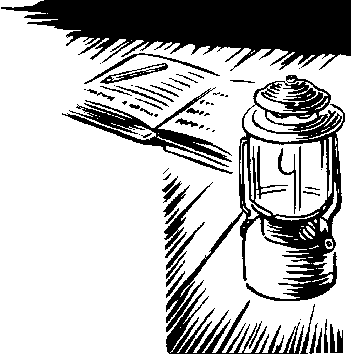
\includegraphics[width=2.9cm]{grafiki/rudy.png}
  \end{center}
\end{wrapfigure}
23 marca zaszła jednak konieczność przeprowadzenia akcji innego typu - aresztowano Rudego (Jana Bytnara), komendanta hufca Południe. Akcja ta, zupełnie precedensowa w skali całej AK, odbyła się 26. marca (17.30 - 17.45) i stała się pierwowzorem dla wszystkich późniejszych akcji dywersji miejskiej. Mimo swej niedoskonałości organizacyjnej (zespół wykonawczy liczył aż 28 osób) stanowiła przełom w sposobach walki z okupantem. Wcześniejsza próba jej przeprowadzenia nie była możliwa, ponieważ brakowało koniecznej decyzji nieobecnego w Warszawie mjr. Lipińskiego. W wyniku akcji zmarli Hubert (Hubert Lenk), Alek (Aleksy Dawidowski) i Buzdygan (Tadeusz Krzyżewicz). Zmarł także odbity Rudy, uwolniono również 23 innych więźniów. W 1944 roku było 18 chorągwi harcerzy (10 000 członków) i 14 chorągwi harcerek (5 000 członkiń). Do tych liczb trzeba dodać harcerzy ze środowisk działających niezależnie od kontynuatorów ZHP (drużyny samodzielne, inne organizacje). Wielu harcerzy zginęło w czasie II wojny światowej, a szczególnym miejscem, masowym grobem było Powstanie Warszawskie. To twoi starsi bracia, pamiętaj o nich. Konspiracyjne harcerstwo było ewenementem na skalę europejską. Trzecim i ostatnim naczelnikiem Sz. Sz. był Leon Marszałek, pełniący tę funkcję od października 1944 (Orsza dostał się wtedy do niewoli niemieckiej) do stycznia 1945 roku (gdy Armia Czerwona wkroczyła do Warszawy). Również w czasie wojny działało harcerstwo poza granicami kraju.

\section{Harcerstwo w PRL i w III Rzeczypospolitej}

Harcerstwo odradzało się żywiołowo w latach 1944 - 45 wszędzie tam, skąd Armia Czerwona wyparła Niemców. Ujawniały się lub powstawały drużyny, organizowały hufce i chorągwie. Wszystko to odbywało się oddolnie, jako że oficjalnie ZHP został powołany do życia decyzją władz oświatowych dopiero 30. grudnia 1944 roku. Nowe władze zdawały sobie sprawę z przydatności ZHP w wychowaniu dzieci i młodzieży, wiedziały jednak dobrze, że jest ono zdominowane przez siły im nieprzychylne, związane z rządem emigracyjnym i AK. Rozpoczęła się więc walka o harcerstwo. Władze utworzyły Tymczasową Naczelną Radę Harcerską, która przygotowała nowe Prawo i Przyrzeczenie oraz Deklarację Ideową. Rekonstrukcja władz centralnych nastąpiła w maju 1945 roku. Nastąpił duży dopływ dawnych instruktorów. Metody pracy opierały się na przedwojennych, a jej płaszczyzny były wynikały z ówczesnej sytuacji kraju: odgruzowanie, służba dla frontu, pomoc rannym, usuwanie pozostałości poniemieckich, pomoc przy żniwach, służba dziecku, pomoc repatriantom, praca dla Ziem Odzyskanych. Harcerstwo liczyło w lipcu 1945 roku ponad 200 000 członków. \begin{wrapfigure}{r}{2cm}
  \begin{center}
    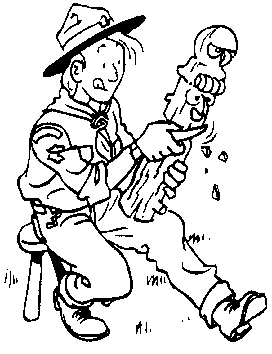
\includegraphics[width=1.94cm]{grafiki/str.png}
  \end{center}
\end{wrapfigure}
Nowych harcerzy przyciągała legenda Szarych Szeregów, jednak dużym problemem był brak kadry - na jednego instruktora przypadało wtedy 450 harcerzy. Był to czas rozwoju harcerskich instytucji zapewniających samowystarczalność - Centrali Dostaw Harcerskich, harcerskich warsztatów wytwarzających umundurowanie. Władze nie zezwalały na Walny Zjazd, gdyż żywiły słuszne obawy, iż zdecydowaną większość będą na nim mieli instruktorzy nie akceptujący władzy przyniesionej do Polski na bagnetach Armii Czerwonej. Starały się o rozszerzenie swych wpływów w ZHP. Wobec trudności z tym związanych, rozpoczęły ofensywę. Jednak starcia na górze w niewielkim stopniu docierały do drużyn.

W końcu 1947 roku Sekretarz Generalny ZHP Pelagia Lewińska przedstawiła projekt zmian organizacyjnych w Związku. Przejawem koncepcji centralnego sterowania programem drużyn była Harcerska Służba Polsce. 
Rezygnując z pracy indywidualnej, podejmowała ona rozmaite zadania społeczne skupione w 4 grupach: Las i rola, Kultura i oświata, Odbudowa kraju oraz Zdrowie i dziecko.
Organizacja rozwijała się liczebnie - w 1948 roku liczyła już 295 500 członków.

Konferencja komendantów i komendantek chorągwi, która odbyła się w dniach 18 - 20 grudnia, przyjęła uchwałę, w której stwierdziła, że obecni na niej instruktorzy zrywają z tradycją harcerską. Odpowiedzią na nią było odejście z ZHP kolejnej grupy instruktorów.

\begin{wrapfigure}{l}{3cm}
  \begin{center}
    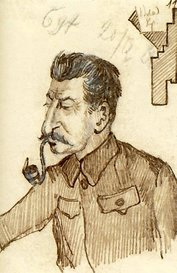
\includegraphics[width=2.9cm]{grafiki/stalin.jpg}
  \end{center}
\end{wrapfigure}
W latach 1848 - 49 zlikwidowano w Polsce wiele organizacji społecznych. Władze uznały, że ZHP jest w swojej obecnej formule nie do zaakceptowania. Postanowiono jednak wykorzystać pozytywny społeczny wizerunek harcerstwa. W styczniu 1949 ograniczono wiek młodzieży harcerskiej do 15 lat. Kontrolę nad ZHP przejmować zaczął Związek Młodzieży Polskiej. W sierpniu Pelagia Lewińska wydała broszurę Walka o nowe harcerstwo, w której oskarżała Związek o służbę na korzyść imperializmu, co było wówczas bardzo poważnym zarzutem. Usuwano kolejnych niewygodnych instruktorów. Na początku 1950 roku Zarząd Główny ZMP, któremu Prezydium przyznano stopnie harcmistrzów, podjął decyzję o przejęciu kierownictwa nad ZHP i ustalił termin jego wcielenia do ZMP na 15 października. Zmieniono Prawo i Przyrzeczenie, symbolikę i mundur. Odrzucono tradycyjne metodykę, formy pracy, rozwiązania programowe i organizacyjne. Zlikwidowano drużyny w szkołach średnich - po ukończeniu podstawówki, harcerze mieli przechodzić do podstawowych struktur ZMP. Odsunięto większość doświadczonych instruktorów. Przewodnikami drużyn zostali etatowi pracownicy szkół. Drużyna skupiała młodzież całej szkoły, a zastępy i ich odpowiedniki - ogniwa - odpowiadały klasie. Organizacja Harcerska ZMP wzorowana była na radzieckiej Organizacji Pionierskiej im. Włodzimierza Lenina, nie uwzględniono jednak odmienności polskich warunków. Harcerze podejmowali prace społeczne, uczestniczyli w wielkich konkursach i imprezach. Zastępy prowadzili nauczyciele, zbiórkami bywały lekcje, a na jednego przewodnika przypadało kilkuset uczniów. Dało to w sumie mało atrakcyjne zbiórki zupełnie nie uwzględniające potrzeb dzieci i młodzieży. Już w roku 1954 OH ZMP poddawana była ostrej krytyce. Otworzyła jej drogę krytyka radzieckiej Organizacji Pionierskiej. Na przełomie maja i czerwca 1955 roku zebrana w Warszawie konferencja programowa wypracowała program, zręby systemu metodycznego i zarys struktury organizacyjnej autonomicznej w ramach ZMP Organizacji Harcerskiej Polski Ludowej. Przywrócono część tradycyjnych metod. To komenda główna OHPL zatwierdziła obowiązującą do dziś odznakę zuchową. Prawdziwe harcerstwo zaczęło odżywać.

8 listopada 1956 roku w Warszawie na naradzie komendantów wojewódzkich OHPL podjęto rezolucję o jej usamodzielnieniu i zaproszono do współpracy wszystkich byłych instruktorów ZHP, którzy gotowi są wychowywać młodzież patriotycznie pod duchowym przewodnictwem PZPR. Stwierdzono iż ocena ZHP zawarta w Walce o nowe harcerstwo była fałszywa i podlega rewizji. Kraj ogarniała polityczna odwilż po latach stalinizmu (Stalin zmarł w 1953 roku). W jej atmosferze 8. grudnia rozpoczęła się w Łodzi Ogólnopolska Narada Działaczy Harcerskich. Drugiego dnia obrad na zaproszenie ONDH (przyjęte przez zaproszonych po wcześniejszej naradzie) przybyła grupa najstarszych i zasłużonych działaczy harcerskich - instruktorów i starszej młodzieży z Sz. Sz. prowadzona przez A. Kamińskiego i S. Broniewskiego. Zgodzili się oni na współpracę. Narada, zwana Zjazdem Łódzkim przyjęła uchwałę o zmianach w organizacji harcerskiej. Zaczął się intensywny okres odtwarzania drużyn, hufców i chorągwi. Trwała normalna praca, przywrócono tradycyjne jej formy, Krzyż Harcerski, lilijkę, nazwę ZHP. Wiek harcerski zwiększono do 16 lat. W 1957 r. powstała Rozgłośnia Harcerska. Powołano specjalną komórkę wydawniczą, prekursora późniejszego Wydawnictwa Harcerskiego Horyzonty, które istniało do 1976 roku. 

W maju ZHP liczył 750 000 członków, ponad połowa drużyn działała na terenach wiejskich. PZPR nie zrezygnowała z wpływów na harcerstwo. Naciskała na dopuszczanie do pracy jedynie wygodnych jej instruktorów (m. in. ateistów). 
Po raz kolejny doprowadzono do odejścia ze Związku wielu doświadczonych instruktorów. 
\begin{wrapfigure}{r}{3cm}
  \begin{center}
    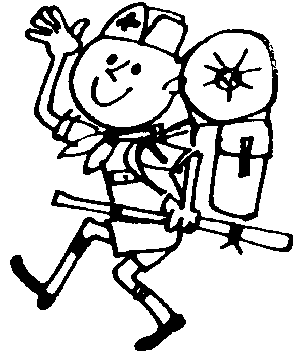
\includegraphics[width=3cm]{grafiki/majzhp.png}
  \end{center}
\end{wrapfigure}Wtedy to wprowadzono pełną etatyzację pracy w centrali, chorągwiach i hufcach mającą uzależnić władze harcerskie od władz politycznych. W 1958 roku powrócono do idei drużyn nieprzetartego szlaku (drużyn dzieci niepełnosprawnych), która została zapoczątkowana w 1920 roku powstaniem pierwszej drużyny głuchoniemych, lecz nie miała wówczas rozmachu, którego dynamicznie nabierała po 1958. W 1984 roku było już 1 696 drużyn NS. Od połowy lat 60. decyzje ważne dla Związku zaczęto podejmować poza nim. Stale ograniczano wiek harcerski. Istniało wiele prób reaktywowania harcerstwa starszego, przeważnie jednak nieudanych. Najważniejsze stały się hasła, deklaracje i przemówienia. W historii harcerstwa i sprawach religii widziano poważne zagrożenia polityczne. Naciskano na masowość ("kierunek 2 miliony") zupełnie nie dbając o jakość. Łamano zasadę dobrowolności działania w ZHP.

W latach 70. bardziej liczyły się długie procesje harcerzy w czasie uroczystości państwowych, niż to, co harcerze chcieli robić. Przedstawicielom szeroko rozumianej władzy udało się wtedy zrobić wszystko, by słowo socjalizm kojarzyło się młodzieży z fałszem i karnie maszerującymi do nikąd kolumnami. Zniesiono wtedy naciski na ograniczenia wiekowe w ZHP, stworzono ciekawe programy starszoharcerskie, lecz zupełnie inaczej wyglądała ich realizacja. Lata 70. to rozwój wielkich akcji, takich jak coroczne alerty Naczelnika ZHP, które wyznaczały jednolite zadania dla wszystkich drużyn. Rozliczne konkursy i turnieje były elementem indoktrynacji politycznej. Pod koniec lat 70. nadmierna ilość akcji i przymus ich podejmowania spowodowały niemal powszechny zanik działania drużynami i zastępami. Wyrosły całe pokolenia instruktorów nie znających samodzielnego działania i zasad metodyki harcerskiej.
Po przemianach politycznych jakie zaszły w kraju po sierpniu 80. roku zrezygnowano z masowości i nadmiernej w Związku dyrektywności programowej. Zaczęto po woli wracać do tradycji. Efektem błędnych koncepcji z lat 60. i 70. był masowy rozpad słabych drużyn i odpływ sporej grupy ludzi przymusowo przypisanych do harcerstwa. 
Narodziły się wtedy ruchy programowo-metodyczne, początkujące proces przemian i odnowy. Od jesieni 1980 roku zaczęły powstawać Kręgi Instruktorów Harcerskich im. Andrzeja Małkowskiego (KIHAM). Celem ruchu była odnowa moralna harcerstwa osiągnięta poprzez przywrócenie autorytetu instruktora. KIHAM-owcy chcieli to osiągnąć poprzez własny przykład. Ich postawa była odwrotnością popularnej wówczas pozy wielkiego działacza. \begin{wrapfigure}{l}{3cm}
  \begin{center}
    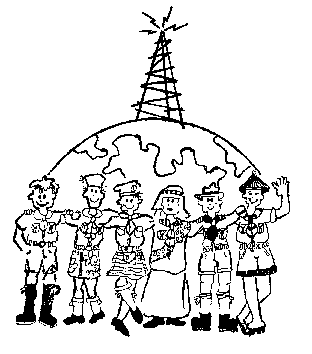
\includegraphics[width=3cm]{grafiki/bts.png}
  \end{center}
\end{wrapfigure}Najważniejszym ich osiągnięciem było stworzenie własnego systemu stopni i sprawności. Drugim ważnym ruchem był Ruch Przyszłość Harcerstwa, którego uczestnicy aktywnie pełnili różne funkcje i zadania w ZHP. Zasięg oddziaływania ruchu rozszerzały publikacje zamieszczane w Na Przełaj. Oba ruchy znacząco wpłynęły na postanowienia podjęte przez VII Zjazd. Podczas stanu wojennego działalność ZHP nie została zawieszona (choć zawieszono wtedy większość związków i stowarzyszeń). Na porządku dziennym znalazła się walka o udział umundurowanych harcerzy w uroczystościach religijnych. Droga do efektywnej pracy harcerskiej była otwarta, choć aparat etatowy był instytucją jedną z najbardziej odpornych na zmiany. Władze Związku wciąż patrzyły na władze państwowe i stosując zachowawczą politykę, bały się wykonać śmiałe kroki prowadzące do głębokich zmian.

Dopiero okrągły stół w roku 1989 i nastanie nowego porządku w Polsce spowodowały prawdziwe, będące powrotem do tradycji, zmiany w Związku dokonane po części na IX (XXVI wg. przywróconej na nim numeracji przedwojennej) Zjeździe w 1989 roku. Przywrócono przedwojenne Prawo i Przyrzeczenie. Ilość harcerzy od lat 80. (1980 - ponad 3 mln.) systematycznie maleje (dziś ok. 400.000). Jednak ta tendencja nie jest obecnie bardzo dynamiczna. W 1989 roku z półkonspiracyjnego, działającego w łonie ZHP, Ruchu Harcerstwa Rzeczypospolitej i Białej Służby (powstałej w 1982 roku na okoliczność II pielgrzymki Jana Pawła II do Polski) powstał Związek Harcerstwa Rzeczypospolitej, organizacja odwołująca się do zasad etyki chrześcijańskiej i tradycji narodowej, uważająca się za kontynuację przedwojennego ZHP (Stanisław Broniewski Orsza uważa się za jej ideowego twórcę, , a także inne organizacje harcerskie (z różnego rodzaju niezależnych ruchów): Związek Harcerstwa Polskiego 1918 (połączył się z ZHR w 1993 roku), Polska Organizacja Harcerska (obecnie połączona z ZHRem), Stowarzyszenie Harcerstwa Katolickiego Zawisza. Z lat biurokracji i centralnego sterowania pozostał zły społeczny obraz harcerstwa oraz zapaść harcerstwa starszego. W 1995 roku w wyniku uchwalenia przez Zjazd ZHP decyzji o zniesieniu wersji Przyrzeczenia Harcerskiego, w której nie składa się ślubu służby Bogu, od Związku odłączył się hufiec Warszawa-Śródmieście i utworzył Stowarzyszenie Harcerskie.